\documentclass{hw_template}

\usepackage{arydshln}

\title{\bfseries Контрольна робота \#2 з Теорії Коливань}
\author{\bfseries Захаров Дмитро}
\date{7 травня, 2025}

\begin{document}

\pagestyle{fancy}

\maketitle

\section{Задача 1}

\begin{problem}
    Визначте асимптотично стійке положення рівноваги системи, яка 
    описується заданим диференціальним рівнянням:
    \begin{equation*}
        \ddot{x} + 5\dot{x} - 0.5x^2 + 0.5 = 0
    \end{equation*}
\end{problem}

\textbf{Розв'язання.} Для початку, знайдемо точки рівноваги цієї системи. Для 
цього введемо нову змінну $y := \dot{x}$. Тоді, маємо:
\begin{equation*}
    \dot{y} + 5y - 0.5x^2 + 0.5 = 0 \implies \dot{y} = -5y + 0.5x^2 - 0.5
\end{equation*}

Таким чином, маємо наступне рівняння вигляду $\dot{\mathbf{z}} = f(\mathbf{z})$, 
де $\mathbf{z} = (x,y)^{\top}$:
\begin{equation*}
    \begin{cases}
        \dot{x} = y \\
        \dot{y} = -5y + 0.5x^2 - 0.5
    \end{cases}
\end{equation*}

Знайдемо, коли праві частини обох рівнянь дорівнюють нулю. Маємо $y=0$, 
а з другого рівняння $x^2=1$. Отже, маємо дві точки рівноваги:
\begin{equation*}
    \mathbf{z}_1 = (1,0)^{\top}, \quad \mathbf{z}_2 = (-1,0)^{\top}
\end{equation*}

Треба з'ясувати, яка з них є асимптотично стійкою. Для цього нам потрібно 
знайти матрицю Якобі $\frac{\partial f}{\partial \mathbf{z}}$. Маємо:
\begin{equation*}
    \frac{\partial f}{\partial \mathbf{z}} = 
    \begin{pmatrix}
        \frac{\partial f_1}{\partial x} & \frac{\partial f_1}{\partial y} \\
        \frac{\partial f_2}{\partial x} & \frac{\partial f_2}{\partial y}   
    \end{pmatrix}
    =
    \begin{pmatrix}
        0 & 1 \\
        x & -5
    \end{pmatrix}
\end{equation*}

На цьому етапі підставимо конкретні точки рівноваги $\mathbf{z}_1$ та
$\mathbf{z}_2$. Якщо підставити $\mathbf{z}_1$, то отримаємо:
\begin{equation*}
    \frac{\partial f}{\partial \mathbf{z}}(\mathbf{z}_1) = 
    \begin{pmatrix}
        0 & 1 \\
        1 & -5
    \end{pmatrix}
\end{equation*}

Характеристичне рівняння $-\lambda(-5-\lambda) - 1 = 0$ або $\lambda^2 +
5\lambda - 1 = 0$. Власні значення $\lambda_{1,2} = -\frac{5}{2} \pm
\frac{1}{2}\sqrt{25+4} = -\frac{5}{2} \pm \frac{\sqrt{29}}{2}$. При 
цьому, одне значення є від'ємним, а інше додатнім. Отже, точка
рівноваги $\mathbf{z}_1$ є сідлом, а отже не є асимптотично стійкою.

Аналогічно, підставляючи $\mathbf{z}_2$, отримаємо:
\begin{equation*}
    \frac{\partial f}{\partial \mathbf{z}}(\mathbf{z}_2) = 
    \begin{pmatrix}
        0 & 1 \\
        -1 & -5
    \end{pmatrix}
\end{equation*}

Характеристичне рівняння $-\lambda(-5-\lambda) + 1 = 0$ або $\lambda^2 +
5\lambda + 1 = 0$. Власні значення $\lambda_{1,2} = -\frac{5}{2} \pm
\frac{1}{2}\sqrt{25-4} = -\frac{5}{2} \pm \frac{\sqrt{21}}{2}$. При цьому,
обидва значення є від'ємними. Отже, точка рівноваги $\mathbf{z}_2$ є
асимптотично стійкою.

\textbf{Відповідь.} Асимптотично стійке положення рівноваги системи описується як $x = -1$, $\dot{x} = 0$.

\newpage 

\section{Задача 2}

\begin{problem}
    Визначте типи точок спокою механічної системи, що описується заданим
    диференціальним рівнянням
    \begin{equation*}
        \ddot{x} = -x + \frac{1}{4}x^3 - \dot{x}
    \end{equation*}
\end{problem}

\textbf{Розв'язання.} Для початку, знайдемо точки рівноваги цієї системи. Для
цього введемо нову змінну $y := \dot{x}$. Тоді, маємо:
\begin{equation*}
    \dot{y} = -x + \frac{1}{4}x^3 - y
\end{equation*}
Таким чином, маємо наступне рівняння вигляду $\dot{\mathbf{z}} = f(\mathbf{z})$,
де $\mathbf{z} = (x,y)^{\top}$:
\begin{equation*}
    \begin{cases}
        \dot{x} = y \\
        \dot{y} = -x + \frac{1}{4}x^3 - y
    \end{cases}
\end{equation*}

Знайдемо, коли праві частини обох рівнянь дорівнюють нулю. Маємо $y=0$, а з
другого рівняння $-x + \frac{1}{4}x^3 = 0$. Корені цього рівняння є $x_1 = 0$,
$x_2=2$, $x_3 = -2$. Тепер лінеаризуємо праву частину системи біля
знайдених точок рівноваги. Для цього нам потрібно знайти матрицю Якобі
$\frac{\partial f}{\partial \mathbf{z}}$. Маємо:
\begin{equation*}
    \frac{\partial f}{\partial \mathbf
    {z}} =
    \begin{pmatrix}
        \frac{\partial f_1}{\partial x} & \frac{\partial f_1}{\partial y} \\
        \frac{\partial f_2}{\partial x} & \frac{\partial f_2}{\partial y}
    \end{pmatrix} = 
    \begin{pmatrix}
        0 & 1 \\
        -1 + \frac{3}{4}x^2 & -1
    \end{pmatrix}
\end{equation*}

Таким чином, підставляючи конкретні точки рівноваги $x_1$, $x_2$ та $x_3$,
знайдемо матрицю Якобі для кожної з них.
\begin{gather*}
    \frac{\partial f}{\partial \mathbf{z}}(\mathbf{z}_1) = 
    \begin{pmatrix}
        0 & 1 \\
        -1 & -1
    \end{pmatrix}, \quad
    \frac{\partial f}{\partial \mathbf{z}}(\mathbf{z}_2) = 
    \begin{pmatrix}
        0 & 1 \\
        2 & -1
    \end{pmatrix} =
    \frac{\partial f}{\partial \mathbf{z}}(\mathbf{z}_3)
\end{gather*}

Знайдемо власні значення матриці Якобі для кожної з точок рівноваги. Для
першої маємо характеристичне рівняння $-\lambda(-1-\lambda) + 1 = 0$ або
$\lambda^2 + \lambda + 1 = 0$. Власні значення $\lambda_{1,2} =
-\frac{1}{2} \pm \frac{i}{2}\sqrt{3}$. Таке значення є комплексним з
від'ємною дійсною частиною. Отже, точка рівноваги $\mathbf{z}_1$ є стійким 
фокусом.

Для другої точки рівноваги маємо характеристичне рівняння
$-\lambda(-1-\lambda) - 2 = 0$ або $\lambda^2 + \lambda - 2 = 0$. Власні
значення $\lambda_1=1$, $\lambda_2=-2$. Одне з значень є додатнім, а інше
від'ємним. Отже, точка рівноваги $\mathbf{z}_2$ є сідлом.

\textbf{Відповідь.} Точка рівноваги $(0,0)$ є стійким фокусом, а точки $(\pm
2,0)$ є сідлом. Зокрема, це підтверджується фазовими портретом, що 
ми зобразили на малюнку \ref{fig:phase_portrait}.

\begin{figure}[h!]
    \centering
    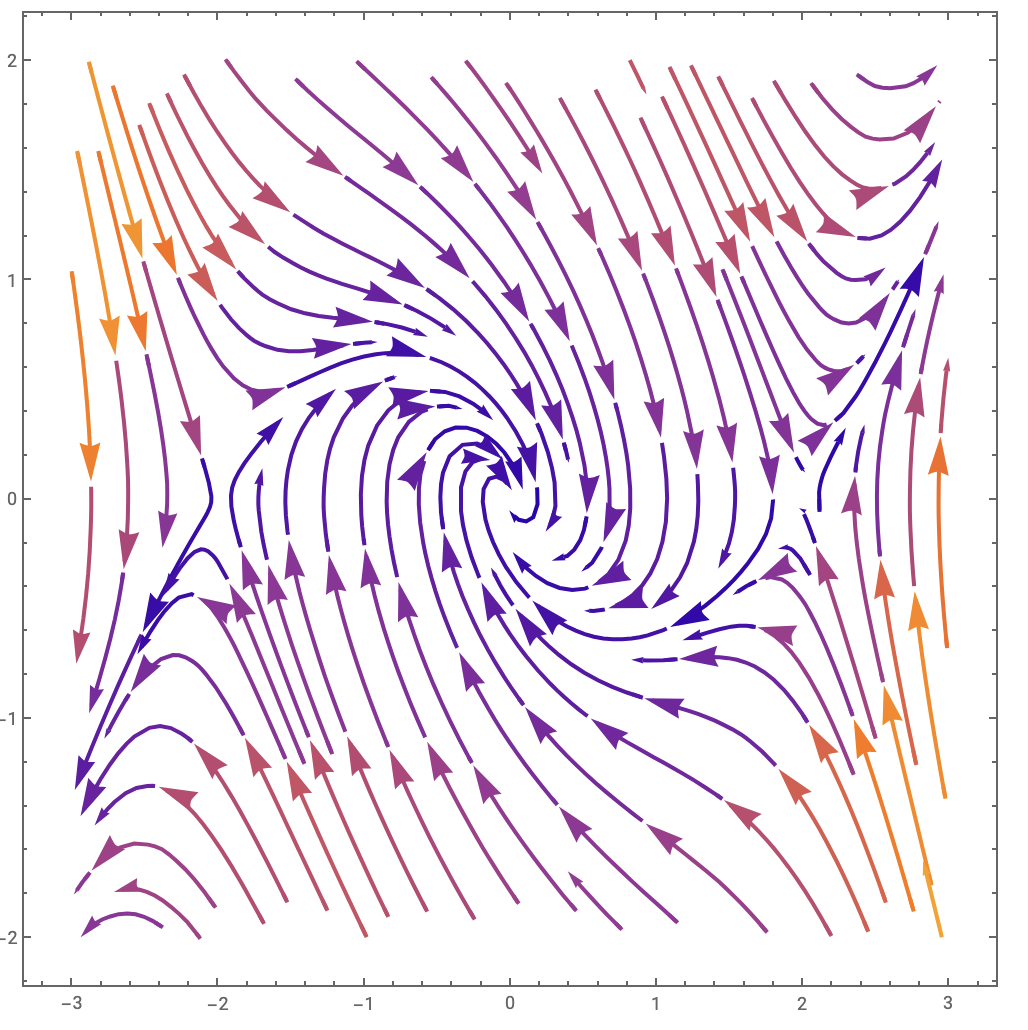
\includegraphics[width=0.5\textwidth]{images/test_2_problem_2.png}
    \caption{Фазовий портрет системи з задачі 2}
    \label{fig:phase_portrait}
\end{figure}

\newpage

\section{Задача 3}

\begin{problem}
    Побудувати фазові портрети нелінійних систем, використовуючи 
    метод лінеаризації в околі особливих точок:
    \begin{equation*}
        \begin{cases}
            \dot{x} = x+y+1 \\
            \dot{y} = y + \sqrt{1+2x^2}
        \end{cases}
    \end{equation*}
\end{problem}

\textbf{Розв'язання.} Для початку, знайдемо точки рівноваги цієї системи.
Для цього розв'яжемо систему рівнянь:
\begin{equation*}
    \begin{cases}
        x+y+1 = 0 \\
        y + \sqrt{1+2x^2} = 0
    \end{cases}
\end{equation*}

Віднімемо від другого перше, тоді матимемо $\sqrt{1+2x^2} = 1+x$. Возведемо
обидві частини до квадрату, матимемо $2x^2+1=x^2+2x+1$, звідки $x^2-2x=0$, а
отже коренями є $x_1=0$, $x_2=2$. Видно, що обидва корені дійсно підходять.
Відповідні точки мають координати $(0,-1)$, $(2,-3)$.

Тепер лінеаризуємо праву частину системи біля знайдених точок рівноваги.
Для цього нам потрібно знайти матрицю Якобі $\frac{\partial f}{\partial
(x,y)}$. Маємо:
\begin{equation*}
    \frac{\partial f}{\partial(x,y)} =
    \begin{pmatrix}
        \frac{\partial f_1}{\partial x} & \frac{\partial f_1}{\partial y} \\
        \frac{\partial f_2}{\partial x} & \frac{\partial f_2}{\partial y}
    \end{pmatrix} = \begin{pmatrix}
        1 & 1 \\
        2x/\sqrt{1+2x^2} & 1
    \end{pmatrix}
\end{equation*}

Таким чином, підставляючи конкретні точки рівноваги $x_1$ та $x_2$, знайдемо
матрицю Якобі для кожної з них.
\begin{gather*}
    \frac{\partial f}{\partial(x,y)}(x_1,y_1) = 
    \begin{pmatrix}
        1 & 1 \\
        0 & 1
    \end{pmatrix}, \quad
    \frac{\partial f}{\partial(x,y)}(x_2,y_2) = 
    \begin{pmatrix}
        1 & 1 \\
        \frac{4}{3} & 1
    \end{pmatrix}
\end{gather*}

Характеристичне рівняння для першої матриці $(1-\lambda)^2 =0$ або $\lambda_1 =
1$ кратності два. Тут доволі складно визначити тип точки, тому проведемо
наступний аналіз: по суті, біля цієї точки система є лінійною, причому виду
$\dot{x}=x+y$ та $\dot{y}=y$. Розв'язок другого рівняння $y(t)=Ae^t$,
підставляючи у перше маємо $\dot{x}=x+Ae^t$, звідки $x(t)=Ate^t + Be^t$. Щоб
отримати краще уявлення про криву, помітимо, що $t = \ln \frac{y}{A}$ і
підставляючи у друге рівняння, маємо $x = y \ln \frac{y}{A} + \frac{B}{A}y$ або
$x=y (\ln ay + b)$. Приблизно це сімейство зображено нижче:
\begin{figure}[h!]
    \centering
    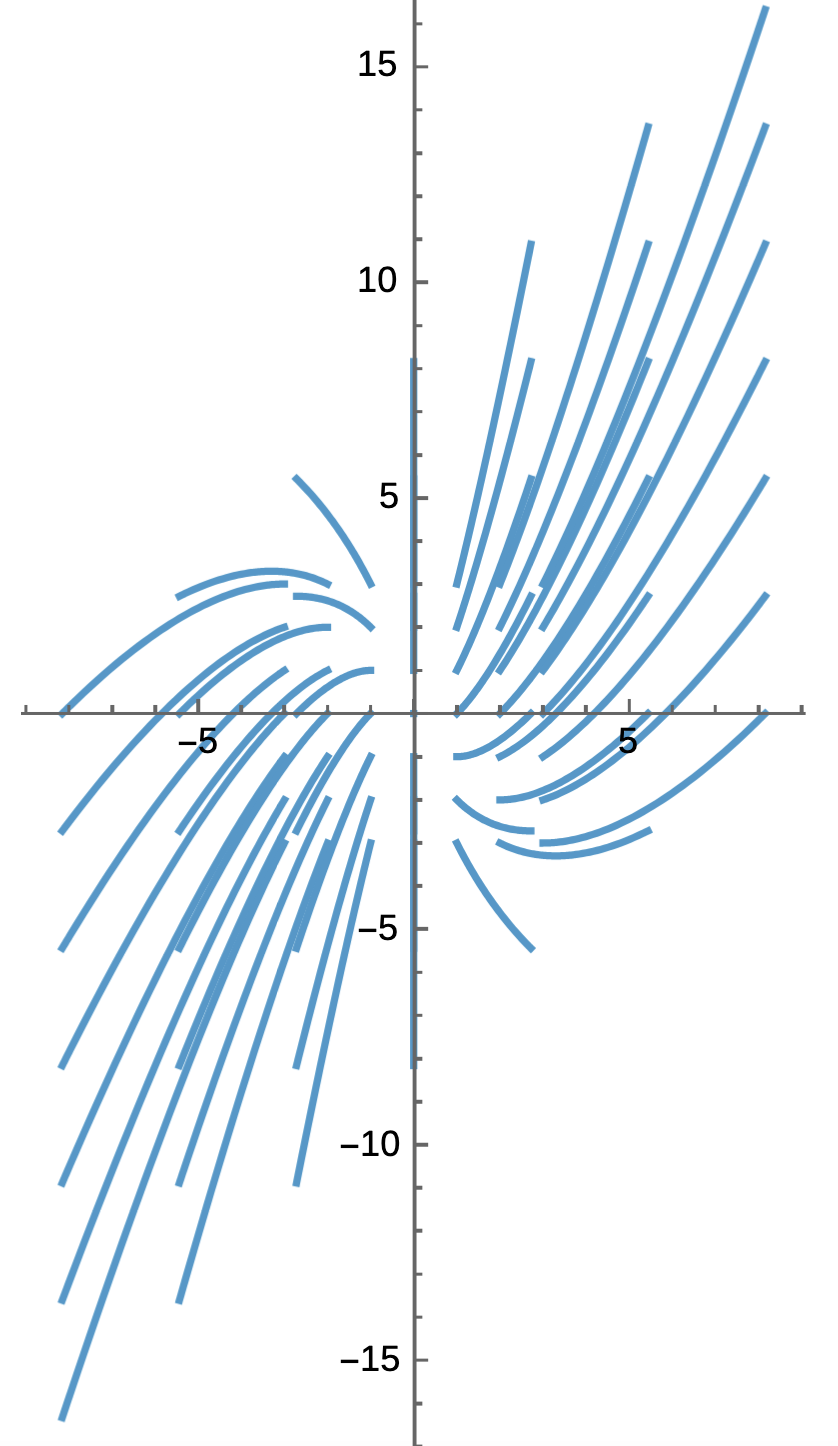
\includegraphics[width=0.35\textwidth]{images/test_2_problem_3_1.png}
    \caption{Приблизний фазовий портрет в околі точки $(0,-1)$}
\end{figure}

Для другої матриці характеристичне рівняння $(1-\lambda)^2 - \frac{4}{3} = 0$ або
$\lambda_1 = 1+\frac{2}{\sqrt{3}}$, $\lambda_2 = 1-\frac{2}{\sqrt{3}}$. Оскільки 
одне значення є додатнім, а інше від'ємним, то точка $(2,-3)$ є сідлом.

\begin{figure}[h!]
    \centering
    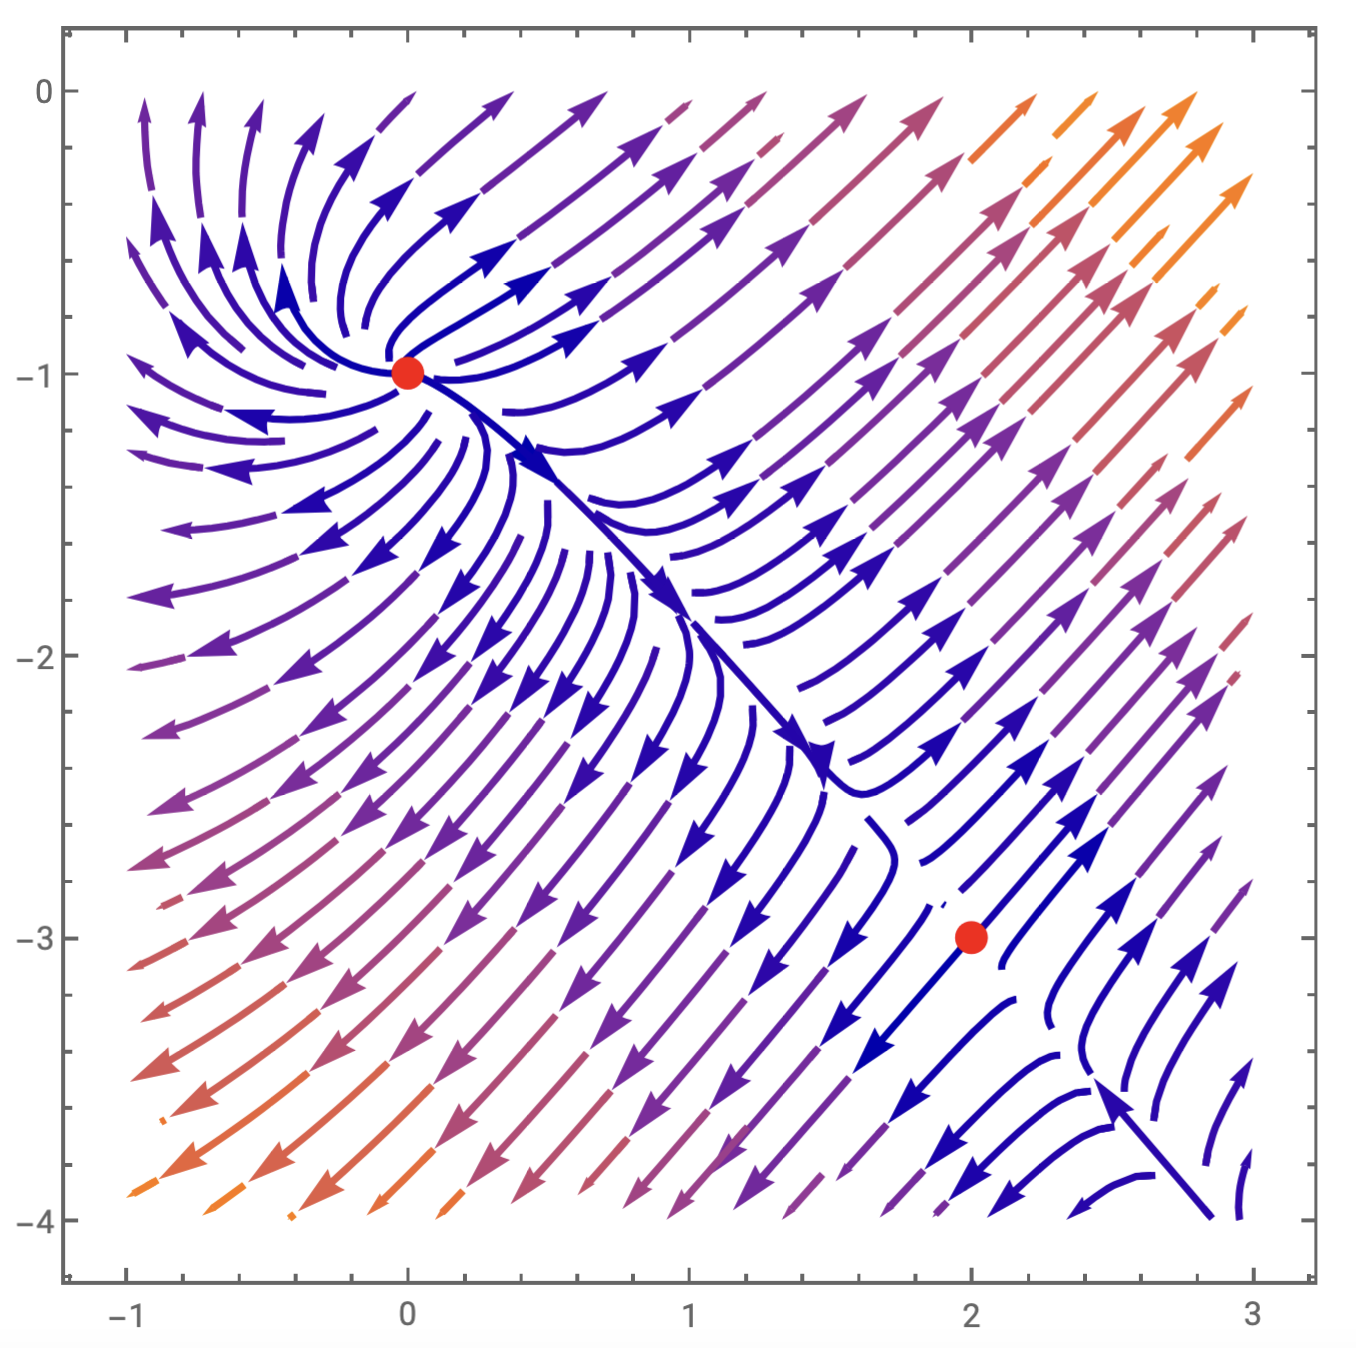
\includegraphics[width=0.5\textwidth]{images/test_2_problem_3_2.png}
    \caption{Фазовий портрет системи з задачі 3}
    \label{fig:phase_portrait_3}
\end{figure}

\newpage

\section{Задача 4}

\begin{problem}
    Побудуйте ескізи усіх можливих типів фазових портретів даної системи з
параметром, якщо $\mu \in \mathbb{R}$. Тут $r,\theta$ --- полярні координати.
\begin{equation*}
    \dot{r} = r(\mu - r^2), \quad \dot{\theta} = 1
\end{equation*}
\end{problem}

\textbf{Розв'язання.} Логічно розглянути два випадки: $\mu > 0$ та $\mu < 0$.
При $\mu > 0$ маємо наступний вид рівняння:
\begin{equation*}
    \dot{r} = r(\sqrt{\mu} - r)(\sqrt{\mu} + r), \quad \dot{\theta} = 1
\end{equation*}

Видно, що при цьому ми маємо лише один граничний цикл $r=\sqrt{\mu}$, а також 
точку спокою в початку координат. Проаналізуємо їх на стійкість. Якщо 
взяти точку з $0 < r_0 < \sqrt{\mu}$, то вираз для похідної $\dot{r} > 0$, а отже 
точка буде наближатись до граничного циклу $r=\sqrt{\mu}$. Якщо при цьому 
початкова точка буде поза кола радіусу $\sqrt{\mu}$, то $\dot{r} < 0$, а отже
точка також буде наближатись до граничного циклу $r=\sqrt{\mu}$. Звичайно, що 
при цьому точка в початку координат є нестійкою. 

При переході через нуль відбувається явище біфуркації. Бачимо, що 
маємо єдину точку спокою в початку координат, яка є стійкою: дійсно, 
вираз $\dot{r} = r(\mu-r^2)$ є завжди від'ємним, бо $r > 0$, а 
$\mu - r^2 < 0$. Таким чином, маємо наступні портрети для $\mu > 0$ та $\mu < 0$, 
що зображені на малюнку \ref{fig:with_friction}.

\begin{figure}
    \begin{tabular}{cc}
      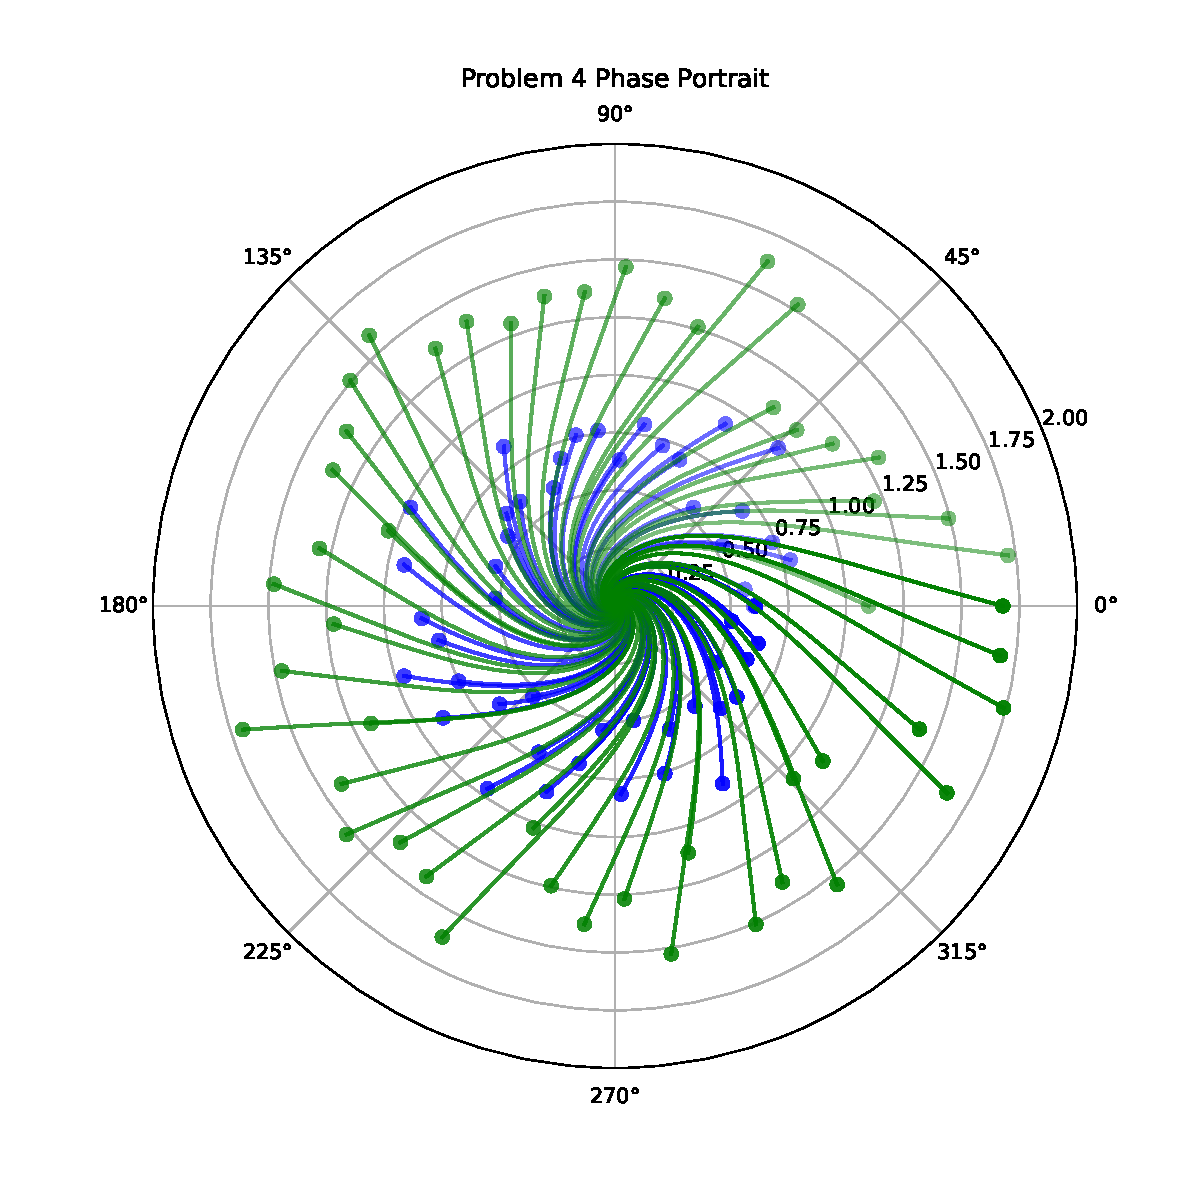
\includegraphics[width=0.5\textwidth]{code/problem_4_-1.0.pdf} &   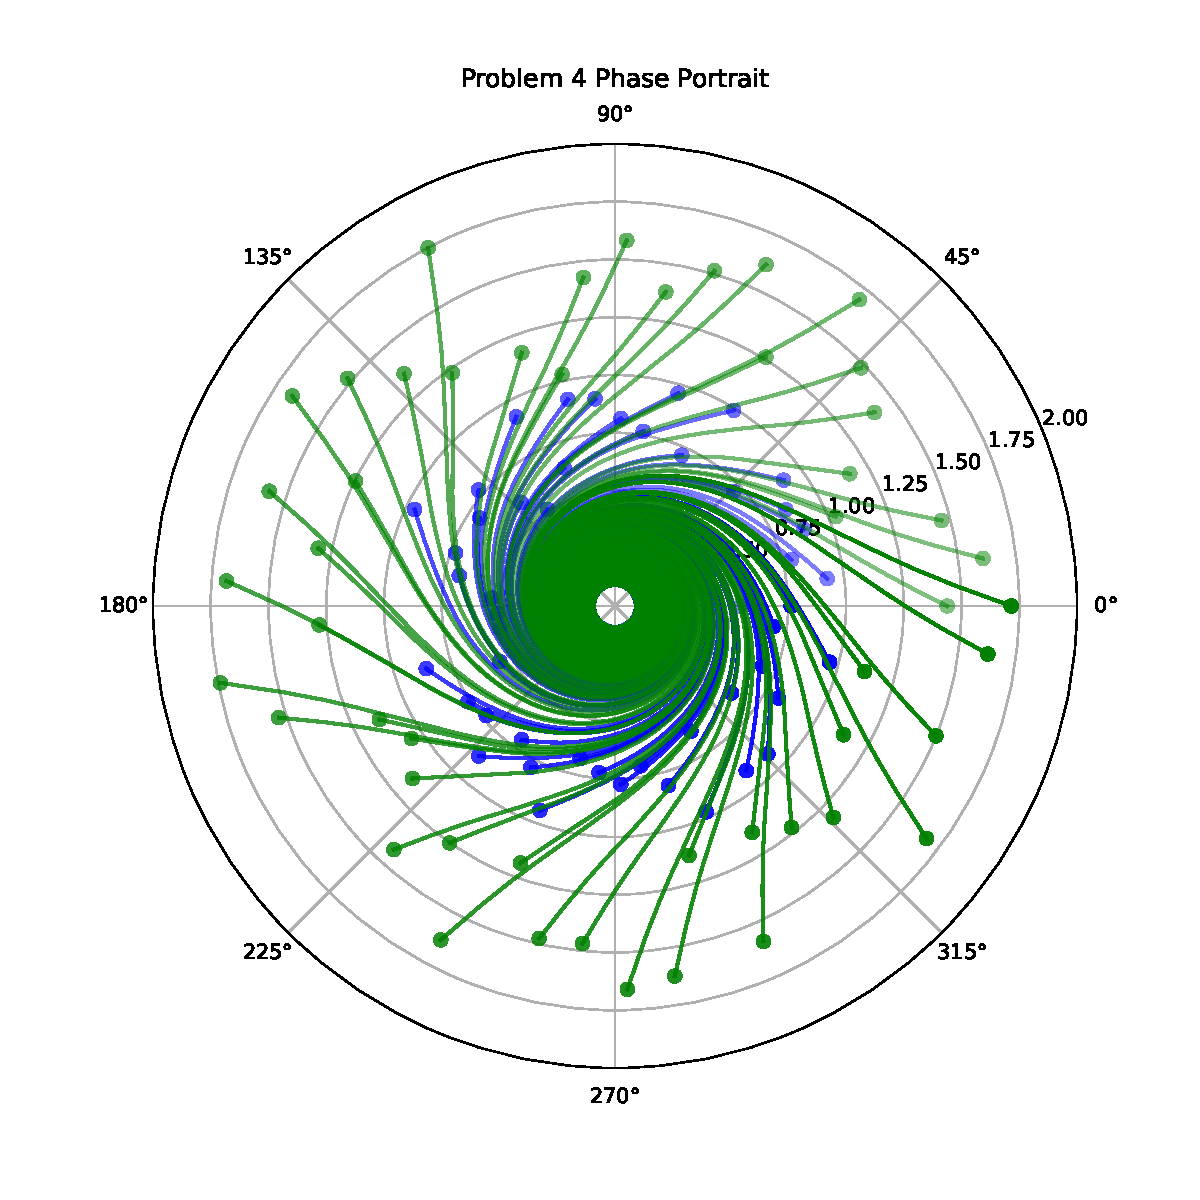
\includegraphics[width=0.5\textwidth]{code/problem_4_0.0.pdf} \\
      $\mu=-1.0$ & $\mu=0.0$ \\
      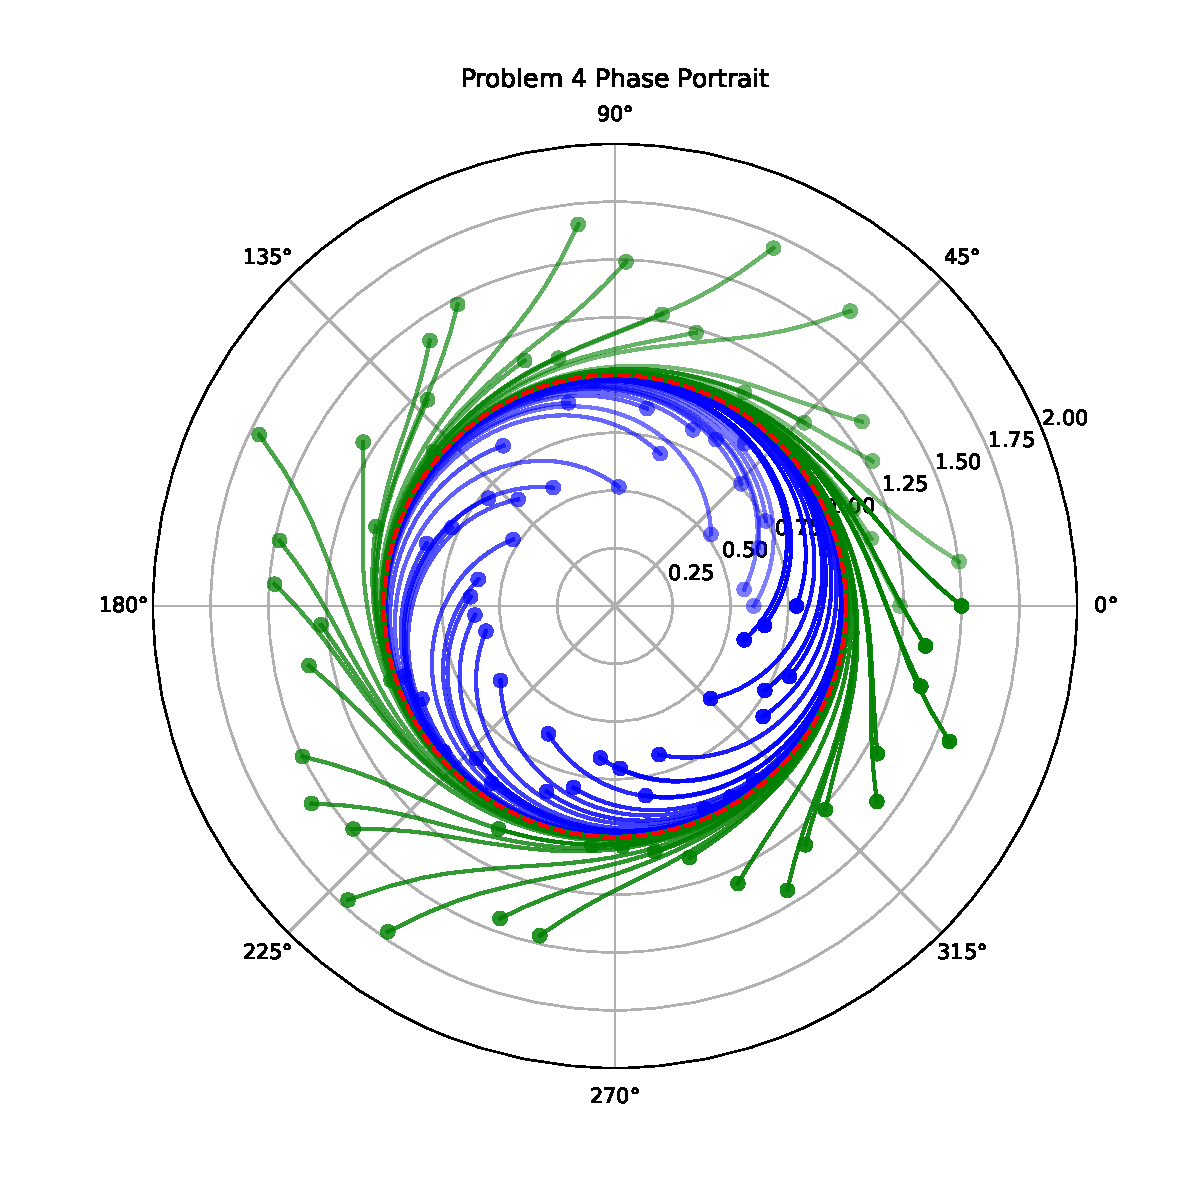
\includegraphics[width=0.5\textwidth]{code/problem_4_1.0.pdf} &   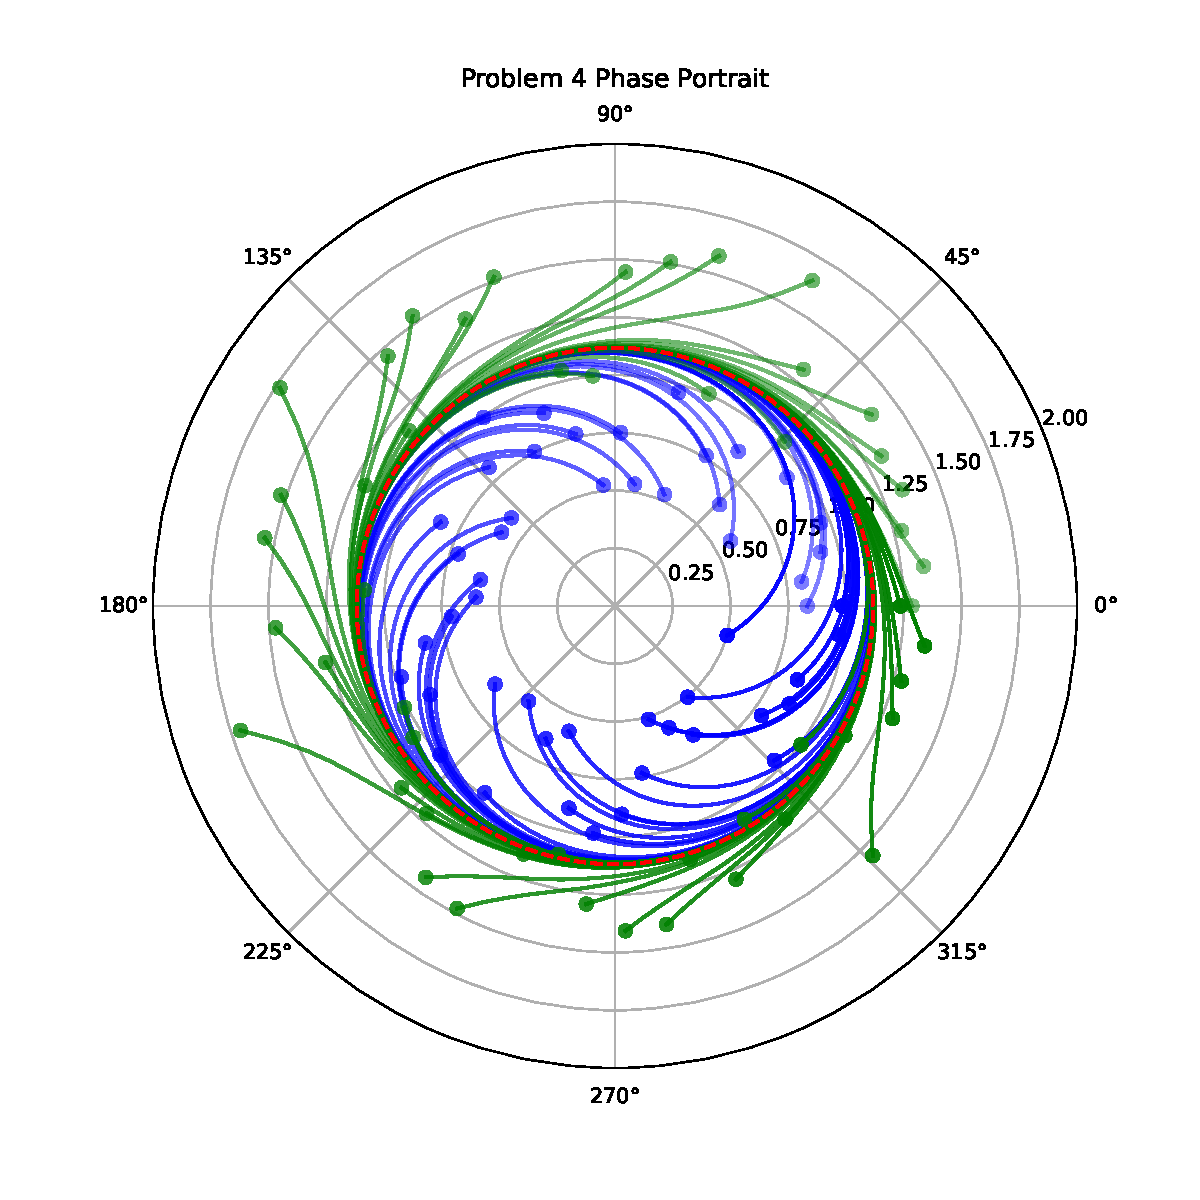
\includegraphics[width=0.5\textwidth]{code/problem_4_1.25.pdf} \\
      $\mu=1.0$ & $\mu=1.25$
    \end{tabular}
    \caption{Фазовий портрет для задачі 4 для різних значень $\mu$.}
    \label{fig:with_friction}
\end{figure}
\end{document}